\section{Results}
\label{sec:results}

\subsection{Gaussian Splatting}
\paragraph{Hyperparameter tuning.} To achieve our first goal, producing a dataset of Gaussian Splats that represent CIFAR-10 images as accurately as possible, we performed a thorough hyperparameter optimization using the \texttt{Optuna} library. 

As expected, the number of Gaussian primitives used was the most influencing factor on reconstruction quality. We tested using $256$, $1024$ and $4096$ Gaussians, and found $1024$ to be a good compromise between reconstruction quality and training efficiency. More interestingly, the opacity regularization factor had a particularly large impact on the optimization result. The initial scale of the Splats also played an important role. More details about the hyperparameter tuning process can be found in the Appendix.

\paragraph{Training and dataset generation.}
In addition to finding optimal hyperparameters for reconstructing the CIFAR-10 images with high fidelity, we found that among the three initialization strategies — random, grid-based and KNN-based — the grid and KNN strategies clearly yielded better reconstructions. For this reason, we decided to generate two datasets of trained Splats for the $60,000$ CIFAR-10 images corresponding to these different initialization strategies.

The rasterized images corresponding to the trained Splats resemble the original images accurately for both grid- and KNN-based initializations, as shown in Fig. \ref{fig:Splat-reconstructions}. While the KNN-based Splats achieved significantly lower losses during training, the grid-based images seem to be visually closer to the original images in most cases, as can be noticed in the images corresponding to the automobile, deer, ship and truck classes. In some instances, the KNN-based Splats achieved a higher accuracy on local details, such as for the frog's eye or the horse's head.

The two generated Gaussian Splat datasets were implemented as \texttt{PyTorch} datasets using a 4 : 1 : 1 split for training, validation, and test sets. The full datasets have a size of approximately 5 GB.

\begin{figure*}
    \centering    \includegraphics[width=1\linewidth]{fig/Splat_reconstruction_comparison.pdf}
    \caption{\textbf{Gaussian Splat Reconstruction of the CIFAR-10 Classes.} Example reconstructions for one of each CIFAR-10 classes. The top row shows the original image, while the middle and lower rows show the Gaussian Splat reconstructions using the grid- and KNN-initializations respectively.}
    \label{fig:Splat-reconstructions}
\end{figure*}

\subsection{Auto-encoding of 2D Splats}
\paragraph{Hyperparameter Tuning.} 
Similarly to the case of the Gaussian Splat dataset generation, we performed a detailed hyperparamter tuning process to find the optimal configuration for each AE variant through \texttt{Optuna}. Interestingly, we found the most critical hyperparameter to be the rate of weight decay, independent of the model architecture and Splat encoding used. Furthermore, we found the random initialization to work better than a Xavier uniform initialization. More details on the results of the hyperparameter tuning for different architectures can be found in the Appendix.

\paragraph{Model comparison.} 
Of the three model architectures that we trained on the whole Splat dataset, the best results were achieved by our convolutional AE. This model was not only able to outperform the simpler deep AE, but also the more sophisticated ResNet-18 AE for all Splat encoding variants. Among the four Splat encodings we tested, the single-channel encoding, where we treated each parameter channel as a separate grayscale image, produced the best results. A comparison of the loss, calculated as the MSE between the input and output Splat encodings, can be found in Fig. \ref{fig:loss-curves}.

\begin{figure}
    \centering    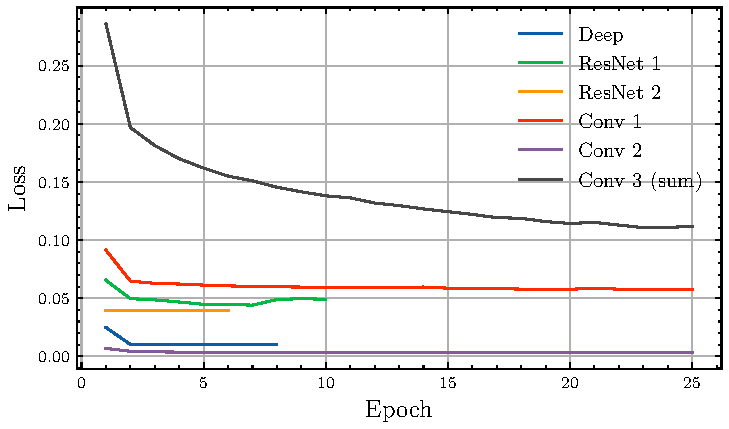
\includegraphics[width=1\linewidth]{fig/loss_curves.pdf}
    \caption{\textbf{Loss Function for Different Model Variants.} The deep model variant used vector encoding, while ResNet 1 and Conv 1 used full-image encoding. Conv 2 and ResNet 2 used single-channel encoding, while Conv 3 trained each parameter independently. In the case of Conv 3, the loss curve shows the sum of individual parameter losses. Some curves are abruptly cut, as the training was stopped early when no improvement was observed.}
    \label{fig:loss-curves}
\end{figure}

\paragraph{Reconstructing the original images.}
Although the MSE between the input and output Splats was extremely close to zero for some models (less than 0.01 in some cases), and the generated input Splats successfully mimic the original images, reconstructing images from AE outputs did not produce entirely satisfactory results. Comparing the renderings created using the outputs of each model, we found that, again, the convolutional model using a single-channel encoding produced the best results. The images reconstructed using the outputs of this model can be found in Fig. \ref{fig:ae-reconstructions}, below the original images from the CIFAR-10 dataset. For comparison, the third row of this figure corresponds to the output of our implementation of a ResNet-18 AE which was trained on raw images instead of Gaussian Splats.

\begin{figure*}
    \centering    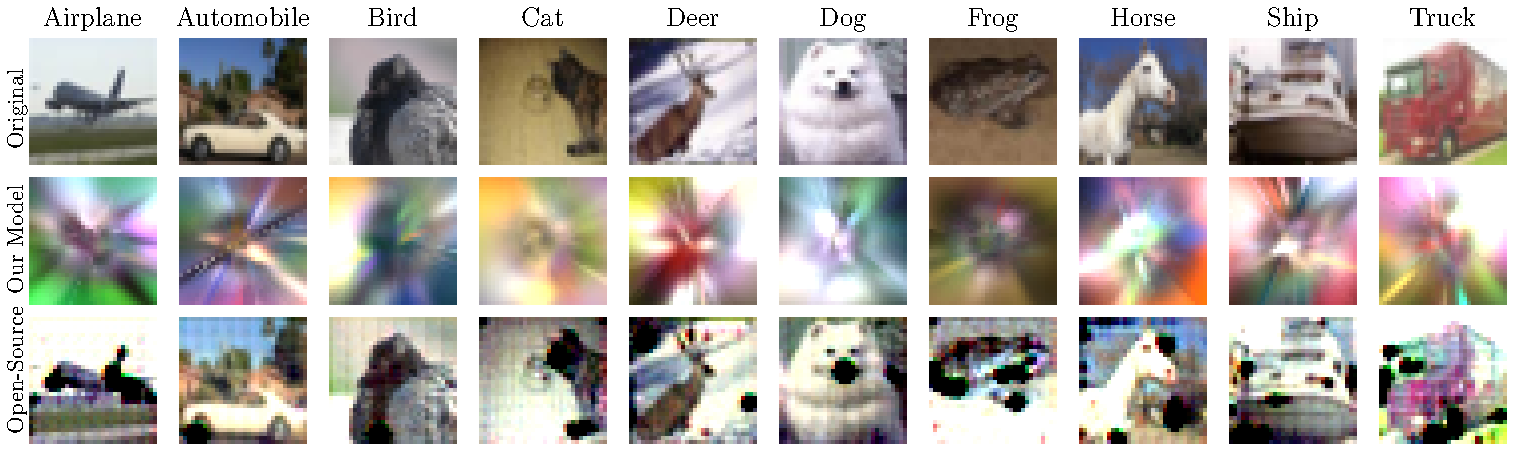
\includegraphics[width=1\linewidth]{fig/reconstruction_comparison.pdf}
    \caption{\textbf{Reconstruction of Autoencoded Images and Gaussian Splats.} The first row on this figure shows 10 random CIFAR-10 images. The second row shows the reconstruction of the CIFAR-10 Splats we generated corresponding to these images, after passing them through our convolutional AE. For comparison, the third row shows the reconstruction of the raw images on the first raw after passing them through our implementation of a ResNet-18 AE.}
    \label{fig:ae-reconstructions}
\end{figure*}

As the convolutional AE with single-channel encoding produced the closest results to the original Splats, we tested training two variants of this model using latent space sizes $4\times4$, corresponding to three Max-Pooling layers, and $8\times8$, corresponding to two Max-Pooling layers. Visually, both model variants produced reconstructions of similar quality, with slightly more accurate colors and structures with a larger latent space, as can be seen in Fig. 9 in the appendix.

\paragraph{Reconstructing individual parameters.}

Considering the lack of a strong visual similarity between the input and output Splats of the AEs despite the low MSE between the tensors representing the Splats, an interesting experiment is visualizing the tensor corresponding to each of the parameters of both input and output Splats. To do this, we visualized the $1024 \times 3$-dimensional parameters as colored images and the $1024$-dimensional parameters as grayscale images. In the case of the quaternions specifying the rotations of the Splats, which have the shape $1024\times4$, we converted them into a three-dimensional rotation matrix, plotted as a colored image. The resulting plots can be found in Fig. \ref{fig:individual-params}.

\begin{figure}
    \centering    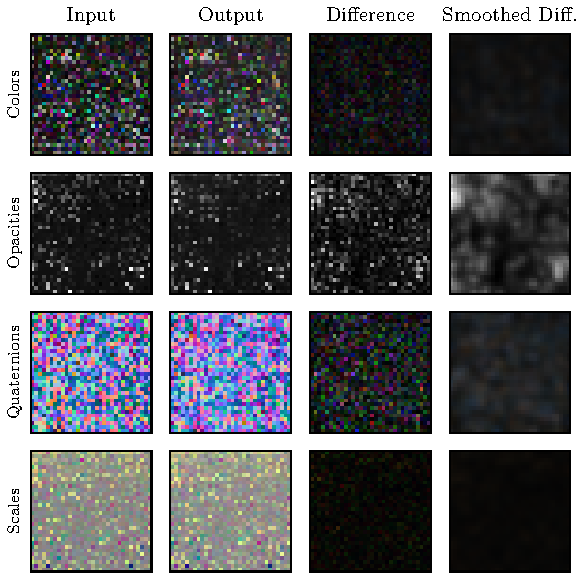
\includegraphics[width=0.97\linewidth]{fig/parameters_individual_viz.pdf}
    \caption{\textbf{Visualization of Individual Parameters of the Input and Output Splats of our Convolutional AE.} Comparison of the tensors corresponding to the individual parameters (colors, opacities, quaternions and scales) of the generated Splats (input) against the same parameters of the autoencoded Splat (output).}
    \label{fig:individual-params}
\end{figure}

This figure reveals that the AEs produced highly similar matrices for every parameter, noticeably almost identical in the case of the colors and scales parameters. This is a particularly interesting result, as it shows that the latent space could represent the most relevant features of the Splats with enough accuracy to reconstruct the parameters with a high fidelity. Furthermore, the latent space of the model was particularly small at a shape of $4\times4$.
